\documentclass[11pt]{article}
\usepackage[T1]{fontenc}
\usepackage[utf8]{inputenc}
\usepackage{lmodern,microtype}
\usepackage[margin=1in]{geometry}
\usepackage{amsmath,amssymb,amsthm,thmtools,bm,mathtools,mathrsfs}
\usepackage{booktabs,array,multirow,tabularx}
\usepackage{graphicx,xcolor}
\usepackage{algorithm}
\usepackage[noend]{algpseudocode}
\usepackage{tikz,pgfplots}
\usetikzlibrary{arrows.meta,positioning,calc,fit,decorations.pathreplacing}
\pgfplotsset{compat=1.18}
\usepackage{enumitem}
\usepackage[numbers,sort&compress]{natbib}
\usepackage{hyperref}
\usepackage[capitalise,nameinlink]{cleveref}

\definecolor{paperblue}{HTML}{17324D}
\definecolor{paperteal}{HTML}{007F83}
\definecolor{paperorange}{HTML}{C8611B}
\definecolor{papergray}{HTML}{6B7280}
\hypersetup{colorlinks=true,linkcolor=paperblue,citecolor=paperteal,urlcolor=paperteal,
  pdftitle={MIST: A GPU Multistage Interior-Point Method for Sum-of-Squares Relaxations of Robot Trajectory Optimization}}

\declaretheorem[name=Theorem,numberwithin=section]{theorem}
\declaretheorem[name=Lemma,sibling=theorem]{lemma}
\declaretheorem[name=Proposition,sibling=theorem]{proposition}
\declaretheorem[name=Corollary,sibling=theorem]{corollary}
\declaretheorem[name=Definition,style=definition,sibling=theorem]{definition}
\declaretheorem[name=Assumption,style=definition,sibling=theorem]{assumption}
\declaretheorem[name=Example,style=definition,sibling=theorem]{example}
\declaretheorem[name=Remark,style=remark,sibling=theorem]{remark}
\crefname{algorithm}{Algorithm}{Algorithms}
\crefname{assumption}{Assumption}{Assumptions}
\crefname{example}{Example}{Examples}
\crefname{remark}{Remark}{Remarks}

% Draft markers. Change \drafttrue to \draftfalse to hide all TODO notes.
\newif\ifdraft \drafttrue
\newcommand{\todo}[1]{\ifdraft{\color{red}\textsf{[TODO: #1]}}\fi}

\newcommand{\R}{\mathbb R}
\newcommand{\Sym}{\mathbb S}
\newcommand{\nnz}{\operatorname{nnz}}
\newcommand{\tr}{\operatorname{tr}}
\newcommand{\Hfull}{\mathscr H_\delta}
\newcommand{\SR}{\mathcal S}
\newcommand{\Oh}{O}

\setlength{\emergencystretch}{2em}

\title{MIST: A GPU Multistage Interior-Point Method for\\
Sum-of-Squares Relaxations of Robot Trajectory Optimization}
\author{xxx\thanks{\todo{affiliation, e-mail}} \and \todo{co-authors}}
\date{\todo{date / venue}}

\begin{document}
\maketitle

\begin{abstract}
Sparse sum-of-squares (SOS) relaxations give certified lower bounds for robot
trajectory optimization, including contact-rich manipulation, but interior-point
methods for the resulting
semidefinite programs spend most of their time forming and factoring a Newton
(Schur-complement) system whose dimension grows with the horizon~$N$. We show
that the temporal locality of the polynomial model reaches this system through
the incidence between coefficient-matching constraints and semidefinite blocks,
and we use this to build an exact, certified elimination scheme. A temporal cut
admits a separator whose size is bounded by the number of monomials of degree at
most $2r$ in the variables shared across the cut. Under bounded temporal support,
an explicit interval ordering yields linear factorization work. For the more
selective hierarchies used in practice, we give a certificate, checkable in
linear time, under which independent elimination of interior components produces
an exact block-tridiagonal system with a global border. The resulting work,
storage and solve bounds depend on accumulated local fronts and retained
interface widths; under uniform local bounds they give $O(N)$ numerical work and
storage and $O(\log N)$ dependency depth. We implement the scheme in SPRINT, a GPU
interior-point solver for SOS relaxations of multistage polynomial optimization
that combines sparse-coordinate Schur assembly, batched
supernodal partial factorization of repeated stage patterns, a small reduced
solve and full-operator residual checks. On contact-rich planning SDPs generated
by SPOT, the hierarchical backend is $1.19$--$1.22\times$ faster than
full-system cuDSS on the same A100, and the reduced solve takes about $1\%$ of
Newton time. On PushBox with horizons up to $80$, SPRINT is $1.5$--$3.2\times$
faster than MOSEK and BRISK for $N\ge20$, and for $N\ge5$ only its solutions
pass a strict $10^{-6}$ check on the original SDP. On a three-dimensional
pendulum problem, SPRINT reaches the same SOS bound as MOSEK $12.3\times$ faster
in solver time.

\end{abstract}

\noindent\textbf{Keywords:} robot trajectory optimization; contact-rich manipulation;
sum-of-squares optimization; semidefinite programming; interior-point methods;
sparse Cholesky factorization; GPU computing.

\section{Introduction}\label{sec:intro}

Polynomial optimization offers a principled route to globally informed robot
trajectory optimization. Once dynamics, contact complementarity and kinematic
constraints are written, or lifted, as polynomial equalities and inequalities,
the moment--sum-of-squares (SOS) hierarchy~\cite{lasserre2001global,parrilo2003semidefinite}
produces semidefinite programs (SDPs) whose optimal values are certified lower
bounds on the trajectory cost. Their solutions often lead to near-optimal
trajectories by extraction or rounding. Relaxations that exploit correlative and
term sparsity~\cite{waki2006sums,lasserre2006convergent,wang2021tssos,wang2022cstssos}
keep long horizons representable. SPOT~\cite{kang2025spot} has demonstrated this
for contact-rich manipulation, related relaxations are tight on several
contact-rich problems~\cite{graesdal2024tight}, and STROM~\cite{kang2024strom}
solves sparse second-order relaxations of polynomial trajectory problems to
certified suboptimality with a first-order (ADMM) SDP solver on the GPU.

Being able to write down such a relaxation does not make it easy to solve.
A sparse trajectory relaxation contains tens of thousands of small
positive-semidefinite (PSD) blocks and hundreds of thousands of equality
constraints; one of our PushT instances with horizon $N=100$ has $259{,}499$
equality rows and $63{,}885$ PSD blocks of order at most $13$. Interior-point
methods (IPMs) remain the method of choice when high accuracy is required, and
most of their time goes into forming and factoring the Schur-complement (Newton)
matrix on the equality constraints. Small PSD blocks do not by themselves make
this matrix cheap to factor. Coefficient-matching rows couple several blocks,
monomials in globally shared variables can span the whole horizon, and an
ordering chosen without knowledge of the model can create large dense fronts.
General-purpose sparse direct solvers on CPUs (as in MOSEK~\cite{mosek}) or GPUs
(as in cuDSS~\cite{cudss}) recover part of this structure through fill-reducing
orderings. They do not know which couplings are temporal, and they cannot
guarantee that a hierarchy remains compatible after the model-specific
simplifications that make elimination cheap. First-order GPU methods such as
STROM's ADMM avoid the Newton system altogether and scale well, but need many
iterations to reach high accuracy. We keep the second-order IPM and make its
Newton system cheap instead.

This paper connects the polynomial model to the graph that the linear solver
actually sees, and uses that connection to build an exact, certified,
GPU-friendly elimination scheme for the IPM Newton system. Our contributions are
as follows.

\begin{enumerate}[leftmargin=*,itemsep=2pt]
\item \textbf{Temporal separators from coefficient matching.} We define the
  \emph{resource graph} of an SOS relaxation, in which every PSD block or free
  variable induces a clique on the coefficient rows it touches. This graph
  contains the sparsity pattern of the Schur matrix and all of its symbolic fill
  (\cref{lem:envelope}). A temporal cut has a separator of size at most
  $\binom{s+2r}{2r}$, where $s$ is the number of polynomial variables shared
  across the cut and $r$ is the relaxation order (\cref{thm:monomial}). Under
  bounded temporal support, an explicit interval ordering gives a path
  decomposition of bounded width, and hence linear factorization work in~$N$
  (\cref{thm:interval}).
\item \textbf{A certified hierarchy with exact condensation.} We give an
  adjacent-interface certificate, checkable in time linear in the size of the
  Schur graph, under which independent elimination of the interior components
  yields an exact block-tridiagonal system with a global border
  (\cref{thm:chain}). The certificate validates aggressive separator pruning and
  temporal coarsening, which are justified algebraically by associativity of
  Schur complements (\cref{prop:assoc}). A compatible hierarchy always exists
  under the modeling assumptions (\cref{thm:spaced}).
\item \textbf{Complexity bounds that depend on the actual fronts.} We bound
  factorization work, storage and solve cost by accumulated local elimination
  fronts, component boundary sizes and retained interface widths
  (\cref{thm:main}). Under uniform local bounds this gives $O(N)$ numerical work
  and storage (\cref{cor:linear}) and $O(\log N)$ dependency depth
  (\cref{cor:depth}). We refine the bounds for unequal interfaces and for the
  supernodal plan that the GPU executes. We also state what the bounds do not
  cover: symbolic setup, the number of outer IPM iterations, and floating-point
  accuracy.
\item \textbf{A GPU interior-point solver.} We present MIST, an
  interior-point solver for SOS relaxations of multistage polynomial
  optimization, and describe its structured backend. It combines sparse-coordinate Schur assembly, certified symbolic
  planning, batched native supernodal partial factorization of repeated stage
  patterns, and a reduced solve by dense Cholesky, cyclic reduction or sparse
  factorization. Every direction is checked against the full operator, and the
  backend falls back to a general factorization when a check fails.
\item \textbf{Experiments at matched and strict accuracy.} On SPOT planning
  SDPs, the hierarchical backend is $1.19$--$1.22\times$ faster than full-system
  cuDSS on the same A100 at $N=30$ and $100$, and the reduced solve takes about
  $1\%$ of Newton time. On PushBox with $N$ up to $80$, MIST is
  $1.5$--$3.2\times$ faster than MOSEK~11 and BRISK~\cite{brisk} for $N\ge20$.
  For $N\ge5$, it is the only one of the three solvers whose solutions pass a
  strict $10^{-6}$ check on the original SDP. On a three-dimensional pendulum
  problem with $N=20$, MIST on one H100 converges $12.3\times$ faster than
  8-thread MOSEK.
\end{enumerate}

The graph-theoretic and block-elimination identities we use are
classical~\cite{rose1976algorithmic,george1973nested,vandenberghe2015chordal},
and linear per-iteration complexity for suitably structured sparse SDPs is known
for other formulations~\cite{zhang2020clique,zhang2024chordal}. We do not claim
the first linear-complexity sparse SDP method. Our contribution is the
specialization of these tools to SOS coefficient incidence, a verifiable
construction of the elimination hierarchy, a cost analysis tied to the
operations the solver executes, and an implementation that turns the analysis
into end-to-end speedups at high accuracy. The analysis uses only the temporal
locality of the relaxation, so it applies to multistage polynomial optimization
in general; in this paper we focus on robot trajectory problems, which motivate
the design and supply all of our test instances.

\paragraph{Organization.}
\Cref{sec:related} reviews related work. \Cref{sec:setting} fixes the SDP and
its Newton system. \Cref{sec:structure} derives temporal separators and an
explicit linear-work ordering, and \cref{sec:hierarchy} develops the certified
hierarchy. \Cref{sec:complexity} gives the complexity bounds, and
\cref{sec:algorithm} describes the GPU solver. \Cref{sec:experiments} reports
the experiments, and \cref{sec:discussion} discusses limitations. The appendices
treat factor reuse across iterations, the correspondence between the analysis and
the implementation, and additional measurements.

\section{Related work}\label{sec:related}

\paragraph{Sparse moment--SOS relaxations.}
The moment--SOS hierarchy~\cite{lasserre2001global,parrilo2003semidefinite}
becomes impractical for long trajectories unless sparsity is exploited.
Correlative sparsity~\cite{waki2006sums,lasserre2006convergent} restricts
monomials to cliques of interacting variables, and term
sparsity~\cite{wang2021tssos,wang2022cstssos} further prunes the monomial bases.
Occupation-measure relaxations of optimal control~\cite{lasserre2008nonlinear}
and recent contact-rich planning relaxations~\cite{graesdal2024tight,kang2025spot}
give the trajectory setting that motivates this work. These papers reduce the
size of the relaxation. We take a fixed sparse relaxation as given and study the
cost of solving its IPM Newton systems.

\paragraph{Certifiable trajectory optimization solvers.}
STROM~\cite{kang2024strom} builds sparse second-order Lasserre relaxations of
polynomial trajectory problems and solves them with cuADMM, a symmetric
Gauss--Seidel ADMM implemented in CUDA, reporting certified suboptimality below
1\% on its benchmarks. TinySDP~\cite{mahajan2026tinysdp} combines PSD-cone
projections with a cached-Riccati ADMM for real-time model predictive control
with nonconvex obstacle constraints on microcontrollers. Both are first-order
methods: each iteration is cheap and parallel, but high accuracy takes many
iterations. MIST is complementary. It keeps the second-order interior-point
method, which reaches high accuracy in a few tens of iterations
(\cref{sec:pushbox}), and makes each Newton step cheap through exact temporal
elimination. On the local side, interior-point solvers for the nonlinear
trajectory problem itself, such as CALIPSO~\cite{howell2022calipso} for conic
and complementarity constraints and Hippo~\cite{zhao2026hippo}, can serve as
the refinement step that turns an extracted relaxation solution into a feasible
trajectory.

\paragraph{Chordal structure and the complexity of sparse SDPs.}
Chordal conversion and matrix completion~\cite{fukuda2001exploiting,nakata2003exploiting,kim2011exploiting,vandenberghe2015chordal}
split large PSD constraints into overlapping small ones, and
first-order methods exploit the same decomposition~\cite{zheng2020chordal}.
\citet{zhang2020clique} showed that dualized clique-tree conversion gives
near-linear-time IPMs for SDPs whose aggregate sparsity graph has small
treewidth. \citet{zhang2024chordal} showed that sparsity of the aggregate graph
alone does not control the Newton-system cost, because the incidence of
constraints on blocks must also be accounted for. Our analysis follows this line
but works directly on the coefficient-matching incidence of a fixed SOS
relaxation. It derives separators from shared monomials and certifies the
hierarchy used by the solver on the assembled Schur graph.

\paragraph{Structured interior-point methods for optimal control.}
For quadratic and nonlinear programs in optimal control, the stagewise structure
of the KKT system is classical: Riccati recursions and block-tridiagonal
factorizations give per-iteration cost linear in the
horizon~\cite{wright1991partitioned,rao1998application,frison2020hpipm}.
In SOS relaxations, the Newton variables are multipliers of coefficient
equations indexed by monomials, not states and controls. Temporal coupling
arises through monomials shared by PSD blocks, and pruning or coarsening can
break a naive stage structure. This is why we need separator bounds and a
certificate before a chain solver can be applied.

\paragraph{Sparse direct methods.}
The relation between elimination orderings and fill is
classical~\cite{rose1976algorithmic,liu1990role}, as are nested
dissection~\cite{george1973nested}, minimum-degree
orderings~\cite{amestoy1996approximate}, multifrontal and supernodal
factorizations~\cite{duff1983multifrontal,chen2008cholmod}, and their
surveys~\cite{davis2016survey}. Block cyclic reduction solves block-tridiagonal
systems with logarithmic depth~\cite{hockney1965fast,heller1976some}. We show
in \cref{prop:ordering} that our hierarchy is one particular elimination
ordering. Its value therefore lies in obtaining a certified ordering and an
efficient GPU execution plan from the model, not in a new factorization
algorithm. NVIDIA cuDSS~\cite{cudss} is the general sparse GPU baseline in our
experiments.

\paragraph{SDP solvers.}
Primal--dual IPMs for SDP~\cite{helmberg1996interior,nesterov1997self,todd1998nesterov},
with Mehrotra-type predictor--corrector steps~\cite{mehrotra1992implementation}
and homogeneous self-dual embeddings~\cite{ye1994homogeneous}, underlie
SeDuMi~\cite{sturm1999sedumi}, SDPT3~\cite{toh1999sdpt3} and
MOSEK~\cite{mosek}. \citet{papp2019sos} optimize directly over the SOS cone
with a nonsymmetric IPM in an interpolant basis, avoiding the SDP reformulation,
and \citet{leijenhorst2024clustered} develop a high-precision primal--dual IPM
for clustered low-rank SDPs arising from polynomial optimization. Parallel and GPU implementations have targeted the dense
Schur complement of general SDPs~\cite{fujisawa2012sdpara}. Low-rank and
first-order methods~\cite{burer2003nonlinear} scale to larger problems but
typically reach lower accuracy, and BRISK~\cite{brisk} is the second CPU
baseline in our experiments. \todo{one sentence describing BRISK's algorithm
and its reference.} On the theoretical side, fast IPMs for SDP and SOS maintain
approximate inverses of the Hessian across
iterations~\cite{jiang2020faster,jiang2022sos}. That work exploits reuse across
iterations, whereas we exploit temporal structure within one iteration;
\cref{app:inverse} discusses how the two might be combined.

\section{Problem setting}\label{sec:setting}

This section fixes the problem class, the SDP that MIST solves, and the linear
system that dominates each interior-point iteration. The rest of the paper is
about solving that linear system quickly and exactly.

\subsection{Multistage polynomial optimization and its SOS relaxation}

We consider polynomial problems whose variables are organized in stages
$\xi_0,\xi_1,\ldots,\xi_N$ and whose objective and constraints couple only
nearby stages:
\begin{equation}\label{eq:pop}
\min_{\xi}\ \sum_{t=0}^{N-1}f_t(\xi_t,\xi_{t+1})
\quad\text{s.t.}\quad
g_{t,a}(\xi_t,\xi_{t+1})\ge0,\quad h_{t,b}(\xi_t,\xi_{t+1})=0,\qquad t=0,\ldots,N-1,
\end{equation}
with polynomial $f_t$, $g_{t,a}$ and $h_{t,b}$. Coupling across a window of
$\ell>2$ stages and a bounded number of global variables are allowed; both enter
the analysis through the parameters of \cref{ass:support}. In robot trajectory
optimization, $\xi_t$ collects the state, control and contact variables of time
step $t$, the equalities encode dynamics, and contact enters through polynomial
complementarity, for example $\lambda\ge0$, $d\ge0$ and $\lambda d=0$, or through
binary mode indicators $\lambda_j^2=\lambda_j$.

Write~\eqref{eq:pop} as $\min\{f(\xi):g_a(\xi)\ge0,\ h_b(\xi)=0\}$. A value $\gamma$
is a certified lower bound if
\begin{equation}\label{eq:sos}
f-\gamma=\sum_c\Bigl(\sigma_{c,0}+\sum_{a}\sigma_{c,a}\,g_a\Bigr)+\sum_b\tau_b\,h_b,
\qquad \sigma_{c,a}=v_{c,a}^{\top}Q_{c,a}v_{c,a},\quad Q_{c,a}\succeq0,
\end{equation}
where $c$ ranges over the cliques of a correlative sparsity
pattern~\cite{waki2006sums,lasserre2006convergent}, $v_{c,a}$ are monomial bases
(possibly pruned by term sparsity~\cite{wang2021tssos,wang2022cstssos}), and
$\tau_b$ are polynomial multipliers. Matching the coefficients of both sides
of~\eqref{eq:sos} gives one affine equation per monomial.

\begin{example}[coefficient matching]\label{ex:matching}
For $p(\xi)=p_0+p_1\xi+p_2\xi^2$ and $v=(1,\xi)$, the identity $p=v^\top Qv$ with
$Q\in\Sym^2_+$ gives three equations, one per monomial $1,\xi,\xi^2$:
$Q_{11}=p_0$, $2Q_{12}=p_1$ and $Q_{22}=p_2$. In a multistage relaxation, a
monomial in the variables of stage $t$ occurs only in the equations of Gram
blocks attached to stages near $t$. This locality is what we exploit.
\end{example}

The lower bound from~\eqref{eq:sos} and the cost of a feasible point recovered
from the relaxation bracket the optimal value of~\eqref{eq:pop}. Whether the
relaxation is tight is a property of the model; the results below concern the cost
of solving a fixed relaxation.

\subsection{The SDP and the interior-point Newton system}

Fixing the relaxation order $r$ and the sparsity rules gives the SDP
\begin{equation}\label{eq:sdp}
\min_{X,\,z}\ \sum_{c=1}^{C}\langle C_c,X_c\rangle+c_z^\top z
\quad\text{s.t.}\quad
\sum_{c=1}^{C}\mathcal A_c(X_c)+Ez=b,\qquad X_c\in\Sym_+^{k_c},\quad z\in\R^{n_f}.
\end{equation}
Each of the $m$ equations is a coefficient-matching equation for one monomial;
$X_c$ are the Gram matrices, of order $k_c$, and $z$ collects the free variables
(the bound $\gamma$ and the coefficients of the multipliers $\tau_b$). We write
$\mathcal A_c(X_c)=(\langle A_i^{(c)},X_c\rangle)_{i=1}^m$.

MIST embeds the free variables in a second-order cone: it adds a scalar $t$ with
zero cost that appears in no equation, and requires $(t,z)\in\mathcal Q^{n_f+1}$.
Every $z$ can be completed by a large enough $t$, so the problem is unchanged, but
all variables now lie in symmetric cones. MIST then applies a primal--dual
interior-point method to the homogeneous self-dual
embedding~\cite{ye1994homogeneous} with Nesterov--Todd
scaling~\cite{nesterov1997self,todd1998nesterov} and Mehrotra
predictor--corrector steps~\cite{mehrotra1992implementation}. Eliminating the
primal and dual directions leaves the normal equations $\mathscr H\,\Delta y=f$ in
the equation multipliers, with
\begin{equation}\label{eq:normal}
\mathscr H=\underbrace{\sum_{c=1}^{C}\mathcal A_c\,\mathcal W_c\,\mathcal A_c^{*}}_{H_{\mathrm{psd}}}
+\widehat E\,W_q^2\,\widehat E^{\top},
\qquad \mathcal W_c(X)=W_cXW_c,\quad \widehat E=[\,0\ \ E\,],
\end{equation}
where $W_c\succ0$ is the scaling of Gram block $c$ and $W_q$ that of the
second-order cone. Entrywise, the first term is
\begin{equation}\label{eq:schur}
(H_{\mathrm{psd}})_{ij}=\sum_{c=1}^{C}\tr\bigl(A_i^{(c)}W_cA_j^{(c)}W_c\bigr).
\end{equation}
The Nesterov--Todd scaling of a second-order cone has the form
$W_q^2=\eta^2(2\bar w\bar w^\top-J)$ with $\eta>0$, $J=\operatorname{diag}(1,-I)$
and $\bar w^\top J\bar w=1$. Because $t$ appears in no equation, the cone's
contribution splits into a sparse part and a single rank-one term:
\begin{equation}\label{eq:operator}
\mathscr H=H_0+uu^\top,\qquad H_0=H_{\mathrm{psd}}+\eta^2EE^\top,\qquad
u=\sqrt2\,\eta\,E\bar w_z,
\end{equation}
where $\bar w_z$ is the trailing part of $\bar w$. The matrix $H_0$ couples two
equations only if they share a Gram block or a free variable. The rank-one term is
dense, which is why it is kept out of every sparsity argument and handled by the
Sherman--Morrison formula (\cref{sec:rankone}). MIST factors a regularized base
\begin{equation}\label{eq:shift}
H_\delta=H_0+\delta I\succ0,\qquad \Hfull=H_\delta+uu^\top,
\end{equation}
with a small shift $\delta\ge0$ chosen by the outer method; every result below
holds verbatim for a diagonal shift.

\paragraph{The linear-algebra task.}
Each IPM iteration assembles $H_\delta$ and $u$, factors $H_\delta$ once, and
solves with a small number $q_{\mathrm{rhs}}$ of right-hand sides: the
homogeneous-embedding column, the predictor, the corrector, and the
Sherman--Morrison column $H_\delta^{-1}u$, so $q_{\mathrm{rhs}}=4$. The corrector
depends on the predictor, so the solves are sequential. Assembling and factoring
$H_\delta$ dominates the cost of an iteration;
\cref{sec:structure,sec:hierarchy,sec:complexity} show how to factor it with work
linear in the horizon, and \cref{sec:algorithm} describes the GPU implementation.
All exactness statements concern this linear system for a fixed shift $\delta$.

\subsection{Notation and computational model}

\Cref{tab:notation} collects the main symbols. We count scalar arithmetic
operations and measure storage in scalar words. Numerical bounds assume that the
symbolic plan and its index maps are available; symbolic analysis is accounted for
separately. A bound called linear in $N$ requires the listed local parameters to
stay bounded as $N$ grows.

\begin{table}[htbp]
\centering
\caption{Main notation.}\label{tab:notation}
\small
\begin{tabular}{@{}lp{0.74\linewidth}@{}}
\toprule
Symbol & Meaning\\
\midrule
$N,\ r$ & horizon and relaxation order\\
$m,\ n_f$ & number of equations and of free variables\\
$\mathcal G=(V,\mathcal E)$ & resource graph on the $m$ equations (\cref{def:resource})\\
$\ell,\ q$ & maximum temporal span of an equation; maximum number of equations first appearing at a stage\\
$n_{\mathrm{var}},\ s$ & variables used by one stage; variables shared across a temporal cut\\
$P$ & monomial interface bound $\binom{s+2r}{2r}$\\
$B,\ g$ & global border equations and $g=|B|$\\
$R_1,\ldots,R_K$ & ordered, disjoint retained interface groups; $p=\max_k|R_k|$\\
$I_j,\ n_j$ & interior connected component and its size\\
$\partial I_j,\ b_j$ & retained neighbors of $I_j$ and their number\\
$d_v,\ w_j$ & later neighbors of interior pivot $v$; maximum later interior neighbors in $I_j$\\
$\Phi_1,\ \Phi_2,\ \mathcal B_2$ & accumulated local-front measures and $\sum_jb_j^2$ (\cref{sec:local})\\
$q_{\mathrm{rhs}}$ & right-hand sides per factorization ($q_{\mathrm{rhs}}=4$ in MIST)\\
\bottomrule
\end{tabular}
\end{table}

\section{Temporal structure of the SOS Newton system}\label{sec:structure}

\paragraph{Overview of the method.}
MIST factors $H_\delta$ in four steps, each justified by one result.
(i) The sparsity of $H_\delta$ is contained in a graph read directly off the
coefficient-matching equations (\cref{lem:envelope}).
(ii) Cutting the horizon between two stages separates this graph by a set of
equations whose size depends only on the variables shared across the cut
(\cref{thm:monomial}); with bounded temporal support this already gives an
ordering with linear work (\cref{thm:interval}).
(iii) MIST keeps a sequence of such interfaces, eliminates everything between
them independently, and obtains an exact block-tridiagonal system on the
interfaces plus a small border; a linear-time certificate guarantees this
structure for the interfaces actually chosen (\cref{thm:chain}).
(iv) The reduced system is solved by dense Cholesky or block cyclic reduction,
and the cost of the whole scheme is bounded by the local elimination fronts and
interface widths (\cref{thm:main}). This section covers steps (i) and (ii),
\cref{sec:hierarchy} step (iii), and \cref{sec:complexity} step (iv).

\subsection{The resource graph}

For each Gram block $c$ and free variable $a$, define the equations they touch:
\begin{equation}\label{eq:support}
\mathcal R_c=\{i:A_i^{(c)}\ne0\},\qquad \mathcal R_a=\{i:E_{ia}\ne0\}.
\end{equation}
We call a Gram block or a free variable a \emph{resource}.

\begin{definition}[resource graph]\label{def:resource}
The resource graph $\mathcal G=(V,\mathcal E)$ has one vertex per equation, and
each resource support $\mathcal R_c$ or $\mathcal R_a$ induces a clique.
\end{definition}

\begin{lemma}[structural envelope]\label{lem:envelope}
The off-diagonal sparsity pattern of $H_\delta$ is contained in $\mathcal G$. For
any elimination order, the fill of $H_\delta$ is contained in the symbolic fill of
$\mathcal G$ for the same order.
\end{lemma}

\begin{proof}
If equations $i$ and $j$ share no Gram block, every term in~\eqref{eq:schur}
vanishes. The term $\eta^2EE^\top$ in~\eqref{eq:operator} couples $i$ and $j$ only
if they share a free variable, and the shift adds nothing off the diagonal. A
pivot updates only pairs of its later neighbors, so induction over the elimination
order gives the fill statement.
\end{proof}

The rank-one term $uu^\top$ is deliberately excluded: it would make $\mathcal G$
complete. Sharing a resource allows a nonzero entry without forcing one, and two
equations using disjoint coordinates of the same Gram block are generally coupled
because $W_c$ is dense. The analysis therefore uses the conservative envelope and
never relies on cancellation.

\subsection{A monomial separator bound}

\begin{assumption}[local coefficient representation]\label{ass:local}
Each equation is identified by a unique monomial $\xi^\alpha$ with
$|\alpha|\le2r$. Each resource is assigned to one stage, and every monomial in its
support uses only variables of that resource. Equations outside this
representation are placed in a border set $B$.
\end{assumption}

At a temporal cut $t$, split the resources into those assigned to stages up to
$t$ and those after $t$. Let $V_L(t)$ and $V_R(t)$ be the variables used by the two
groups, and let
\begin{equation}\label{eq:shared}
S_t=V_L(t)\cap V_R(t),\qquad s_t=|S_t|.
\end{equation}
Let $\mathcal Q_t$ be the equations outside $B$ that touch resources on both sides.

\begin{theorem}[monomial interface bound]\label{thm:monomial}
Under \cref{ass:local}, removing $\mathcal Q_t$ disconnects the equations used only
on the left from those used only on the right in $\mathcal G[V\setminus B]$, and
\begin{equation}\label{eq:monomial}
|\mathcal Q_t|\le\binom{s_t+2r}{2r}.
\end{equation}
\end{theorem}

\begin{proof}
An equation in $\mathcal Q_t$ is a monomial occurring in a resource on each side,
so its variables lie in $V_L(t)\cap V_R(t)=S_t$. There are exactly
$\binom{s_t+2r}{2r}$ monomials of degree at most $2r$ in $s_t$ variables, and each
equation is a distinct monomial. Any remaining equation touches resources on one
side only. An edge between a left-only and a right-only equation would mean a
shared resource, which lies on one side and contradicts the other equation being
exclusive to the opposite side.
\end{proof}

The bound depends on the variables shared across the cut, not on the size of a
stage: a stage with $n_{\mathrm{var}}$ variables can carry up to
$\binom{n_{\mathrm{var}}+2r}{2r}$ equations, but the interface it creates is
controlled by $\binom{s_t+2r}{2r}$, and term sparsity typically keeps fewer
monomials still. In PushT (\cref{sec:experiments}), consecutive stages share only
the planar pose $(\cos\theta,\sin\theta,s_x,s_y)$, so $s_t=4$ and $r=2$ give at
most $\binom{8}{4}=70$ interface equations per cut, although each stage uses 22
variables. The interfaces MIST retains at $N=100$ after pruning and coarsening
have 37 equations on average.

\subsection{Bounded temporal support and an explicit linear-work ordering}

For an equation $i\notin B$, let $\mathcal T_i$ be the stages of the resources it
touches, and define its occurrence interval
\begin{equation}\label{eq:interval}
J_i=[a_i,b_i],\qquad a_i=\min\mathcal T_i,\quad b_i=\max\mathcal T_i.
\end{equation}

\begin{assumption}[bounded temporal support]\label{ass:support}
There are constants $\ell,q,g$, independent of $N$, such that $|B|=g$, every
equation $i\notin B$ satisfies $b_i-a_i+1\le\ell$, and at most $q$ equations first
appear at any one stage.
\end{assumption}

For~\eqref{eq:pop}, a variable used by stages $t$ and $t+1$ only produces
monomials of span at most two, and a stage with $n_{\mathrm{var}}$ variables gives
$q\le\binom{n_{\mathrm{var}}+2r}{2r}$. Monomials in global variables alone, such
as the constant monomial, go to $B$.

\begin{theorem}[interval path decomposition]\label{thm:interval}
Under \cref{ass:support}, $\mathcal G$ has a path decomposition of width at most
$\ell q+g-1$. Eliminating the equations outside $B$ in nondecreasing order of
$b_i$, followed by $B$, costs
\begin{equation}\label{eq:interval-cost}
W_{\mathrm{chol}}=O\bigl(Nq(\ell q+g)^2+g^3\bigr),\qquad
M_{\mathrm{chol}}=O\bigl(Nq(\ell q+g)+g^2\bigr).
\end{equation}
\end{theorem}

\begin{proof}
For each stage $t$, form the bag $X_t=B\cup\{i:t\in J_i\}$. Two non-border
equations sharing a resource lie together in the bag of that resource's stage, and
border equations lie in every bag, so all edges are covered. The bags containing a
non-border equation form its interval $J_i$, which gives the running-intersection
property. If $t\in J_i$, then $a_i$ is one of the $\ell$ stages ending at $t$, so
$|X_t|\le\ell q+g$.

For the ordering, consider the supergraph in which two non-border equations are
adjacent whenever their intervals intersect and border equations are adjacent to
everything. When the remaining equation with the smallest right endpoint $b_i$ is
eliminated, all of its remaining neighbors contain $b_i$ in their intervals, so
they already form a clique with $B$. The order creates no fill in the supergraph,
hence the fill of $\mathcal G$ stays inside it. Each of the at most $Nq$
non-border pivots has a front of size at most $\ell q+g$, costing
$O((\ell q+g)^2)$ work and $O(\ell q+g)$ storage; the border costs $O(g^3)$ and
$O(g^2)$.
\end{proof}

\Cref{thm:interval} is the multistage analogue of the classical link between
treewidth and factorization cost, with the decomposition read off the SOS model;
as noted by \citet{zhang2024chordal}, it is the incidence of constraints on
blocks, not the aggregate sparsity of the Gram matrices, that controls the
Newton-system cost. The theorem guarantees its own explicit order, not the result
of a generic AMD or nested-dissection ordering. It is also pessimistic: it charges
every pivot the largest bag, even though most equations of a stage belong to small
substructures. The hierarchy of the next section removes this pessimism.

Separators at different cuts need not be disjoint, since a monomial can persist
across several cuts, and separators chosen independently at each cut need not
produce a block-tridiagonal reduced system. The next section therefore makes
compatibility an explicit, checkable condition on the interfaces the solver uses.

\section{Certified hierarchical elimination}\label{sec:hierarchy}

\subsection{Retained interfaces and the adjacent-interface certificate}

Choose disjoint retained sets and let $I$ be their complement:
\begin{equation}\label{eq:retained}
R=B\mathbin{\dot\cup}R_1\mathbin{\dot\cup}\cdots\mathbin{\dot\cup}R_K,\qquad I=V\setminus R.
\end{equation}
Let $I_1,\ldots,I_J$ be the connected components of $G[I]$, with retained
boundaries $\partial I_j=N_G(I_j)\cap R$. The groups $R_k$ are indexed
consecutively in the retained order. Stage indices can have gaps after pruning
or coarsening, so they cannot replace these compact indices when testing
adjacency.

\begin{definition}[adjacent-interface certificate]\label{def:certificate}
The retained partition is \emph{certified} if
\begin{enumerate}[label=(\roman*),itemsep=1pt]
\item every edge of $G[R]$ with both endpoints outside $B$ joins vertices in the
  same group or in two consecutive groups; and
\item for every interior component, $\partial I_j\setminus B\subseteq R_k\cup R_{k+1}$
  for some $k$. A component may also touch a single group or none.
\end{enumerate}
\end{definition}

Given adjacency lists, the certificate can be checked in $O(m+|\mathcal E|)$
time: find the components of $G[I]$, scan their incident edges while recording
the smallest and largest compact group index met, and check the retained-to-retained
edges in the same scan. No table indexed by components and retained rows is
needed. With the ordering $I_1,\ldots,I_J,R$, the operator has the block-arrow
form
\begin{equation}\label{eq:arrow}
H_\delta=\begin{bmatrix}
A_1&&&G_1\\&\ddots&&\vdots\\&&A_J&G_J\\G_1^\top&\cdots&G_J^\top&D
\end{bmatrix},
\end{equation}
in which $G_j$ has nonzero columns only on $\partial I_j$.

\begin{theorem}[exact chain condensation]\label{thm:chain}
Suppose $H_\delta\succ0$ and \cref{def:certificate} holds. Then
\begin{equation}\label{eq:reduced}
S=D-\sum_{j=1}^{J}G_j^\top A_j^{-1}G_j\succ0
\end{equation}
is block tridiagonal on $R_1,\ldots,R_K$, with arbitrary coupling to $B$. For
every right-hand side $f$, solving $H_\delta x=f$ is equivalent to
\begin{equation}\label{eq:condense}
\widehat f_R=f_R-\sum_jG_j^\top A_j^{-1}f_j,\qquad
Sx_R=\widehat f_R,\qquad
x_j=A_j^{-1}(f_j-G_jx_R).
\end{equation}
\end{theorem}

\begin{proof}
Each $A_j$ is a principal submatrix of an SPD matrix and is therefore
invertible; block elimination gives~\eqref{eq:reduced} and~\eqref{eq:condense}.
The update from component $j$ is supported on $\partial I_j\times\partial I_j$.
By condition~(ii), it can fill only one retained group, two adjacent groups and
the border. Condition~(i) gives the same restriction for $D$. Hence no two
nonadjacent groups become coupled. Positive definiteness follows from the
Schur-complement property of SPD matrices.
\end{proof}

\Cref{eq:reduced} is an algebraic description. The implementation forms neither
$A_j^{-1}$ nor $A_j^{-1}G_j$; partial elimination of a local augmented matrix
produces the retained-front update directly (\cref{sec:local-factor}).
\Cref{fig:hierarchy} illustrates the structure.

\begin{figure}[htbp]
\centering
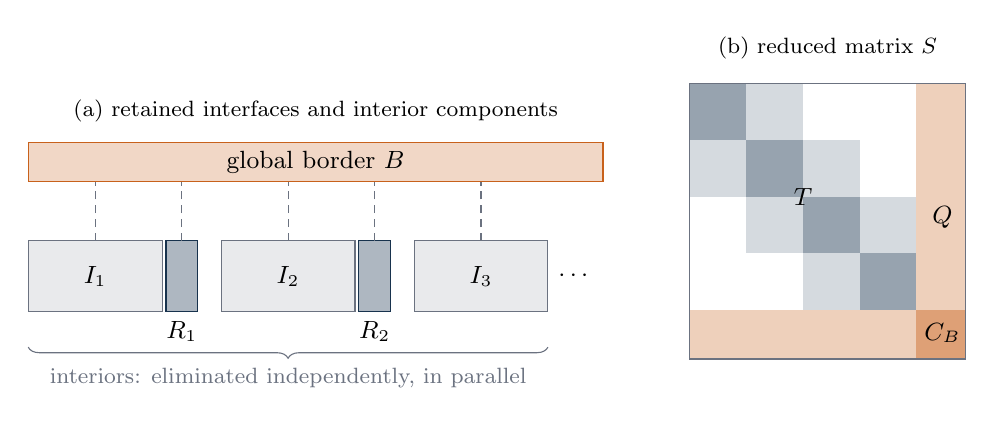
\begin{tikzpicture}[x=1cm,y=1cm,font=\small]
  % (a) graph view
  \foreach \x/\lab in {0/1,2.45/2,4.9/3}{
    \draw[fill=papergray!15,draw=papergray] (\x,0) rectangle ++(1.7,0.9);
    \node at (\x+0.85,0.45) {$I_{\lab}$};
  }
  \foreach \x/\lab in {1.95/1,4.4/2}{
    \draw[fill=paperblue!35,draw=paperblue] (\x-0.2,0) rectangle ++(0.4,0.9);
    \node[below] at (\x,0) {$R_{\lab}$};
  }
  \node at (6.95,0.45) {$\cdots$};
  \draw[fill=paperorange!25,draw=paperorange] (0,1.65) rectangle (7.3,2.15);
  \node at (3.65,1.9) {global border $B$};
  \foreach \x in {0.85,3.3,5.75,1.95,4.4}{
    \draw[densely dashed,papergray] (\x,0.9) -- (\x,1.65);
  }
  \draw[decorate,decoration={brace,mirror,amplitude=4pt},papergray]
    (0,-0.45) -- (6.6,-0.45) node[midway,below=4pt,align=center,font=\footnotesize]
    {interiors: eliminated independently, in parallel};
  \node[font=\footnotesize] at (3.65,2.55) {(a) retained interfaces and interior components};
  % (b) reduced matrix
  \begin{scope}[shift={(8.4,-0.6)}]
    \def\n{4}\def\w{0.72}
    \draw[papergray] (0,0) rectangle (3.5,3.5);
    \foreach \k in {0,...,3}{
      \fill[paperblue!45] ({\k*\w},{3.5-(\k+1)*\w}) rectangle ++(\w,\w);
    }
    \foreach \k in {0,...,2}{
      \fill[paperblue!18] ({(\k+1)*\w},{3.5-(\k+1)*\w}) rectangle ++(\w,\w);
      \fill[paperblue!18] ({\k*\w},{3.5-(\k+2)*\w}) rectangle ++(\w,\w);
    }
    \fill[paperorange!30] (4*\w,{3.5-4*\w}) rectangle (3.5,3.5);
    \fill[paperorange!30] (0,0) rectangle (4*\w,{3.5-4*\w});
    \fill[paperorange!60] (4*\w,0) rectangle (3.5,{3.5-4*\w});
    \draw[papergray] (0,0) rectangle (3.5,3.5);
    \node at (1.44,2.06) {$T$};
    \node at (3.21,1.8) {$Q$};
    \node at (3.21,0.33) {$C_B$};
    \node[font=\footnotesize,align=center] at (1.75,3.95) {(b) reduced matrix $S$};
  \end{scope}
\end{tikzpicture}
\caption{The certified hierarchy. (a) Removing the retained groups $R_k$ and the
border $B$ leaves interior components $I_j$ that touch at most two consecutive
groups. (b) Eliminating the interiors exactly yields a block-tridiagonal chain
$T$ on $R_1,\ldots,R_K$ coupled to a small dense border block $C_B$.}
\label{fig:hierarchy}
\end{figure}

\subsection{Separator pruning and temporal coarsening}

Let $\SR_R(H)$ denote the Schur complement of $H$ onto $R$, obtained by
eliminating $V\setminus R$.

\begin{proposition}[associativity of Schur complements]\label{prop:assoc}
If $R'\subseteq R$ and $H\succ0$, then $\SR_{R'}\bigl(\SR_R(H)\bigr)=\SR_{R'}(H)$.
\end{proposition}

\begin{proof}
For fixed $x_R$,
\begin{equation}\label{eq:minform}
x_R^\top\SR_R(H)\,x_R=\min_{x_{V\setminus R}}x^\top Hx.
\end{equation}
Minimizing further over $x_{R\setminus R'}$ is the same as minimizing the
original form over $x_{V\setminus R'}$. The quadratic forms coincide, and the
minimizers are unique because $H\succ0$.
\end{proof}

\Cref{prop:assoc} justifies two simplifications. \emph{Carry pruning} absorbs
separator rows that terminate in a one-sided branch into a neighboring interior,
and \emph{temporal coarsening} removes selected cuts so that several stages
form one interior. In both cases the new partition must again satisfy
\cref{def:certificate} before a chain solver is used. The heuristic that proposes
candidates is not trusted; only the certificate is. Reducing $|R|$ does not
necessarily reduce total work, because larger interiors can create larger
local fronts (\cref{sec:select}).

\subsection{Existence of a compatible hierarchy}

The certificate is not only an a posteriori test: under the modeling assumptions
a compatible hierarchy can be constructed directly.

\begin{theorem}[spaced-cut construction]\label{thm:spaced}
Suppose \cref{ass:local,ass:support} hold. Choose an integer $h\ge\ell$, divide
the stages into consecutive slabs of at most $h$ stages, place cuts at
$h,2h,\ldots$ strictly before $N$, and retain the rows $Q_t$ of
\cref{thm:monomial} at each cut. Then the retained sets are pairwise disjoint
and, after empty groups are removed, satisfy \cref{def:certificate}. Every
interior component lies in one slab. If each cut shares at most $s$ variables
and $P=\binom{s+2r}{2r}$, then
\begin{equation}\label{eq:spaced}
p\le P,\qquad b_j\le2P+g,\qquad n_j\le hq,\qquad K\le N/h.
\end{equation}
\end{theorem}

\begin{proof}
A row crossing the cuts at $t$ and $t+h$ has $a_i\le t$ and $b_i\ge t+h+1$, so
its span is at least $h+2>\ell$, which contradicts \cref{ass:support}; hence no
non-border row is retained twice. A non-retained row crosses no cut, so all of
its resources lie in one slab, and rows in different slabs share no resource.
Every interior component therefore lies in one slab, and since all of its rows
first appear in that slab, it has at most $hq$ vertices.

A retained neighbor of a component shares a resource inside the component's slab
and crosses its own cut. If that cut were not a boundary cut of the slab, the
row would also cross the boundary cut lying in between, and would be retained
twice. Hence a component touches only the two boundary groups of its slab and
$B$. Finally, two retained rows at nonconsecutive cuts cannot share a resource:
at a cut strictly between them, the earlier row has all of its resources on the
left and the later row all of its resources on the right, since otherwise one of
them would cross two cuts. Empty groups have no incident edges and can be
removed. The bounds follow from \cref{thm:monomial}, the slab argument and the
number of cuts.
\end{proof}

The construction proves existence and correctness. It does not minimize fronts,
and the solver usually retains smaller cuts and prunes more aggressively, using
the certificate to validate each choice.

\subsection{The rank-one correction}\label{sec:rankone}

Let $v=H_\delta^{-1}u$. The Sherman--Morrison identity gives
\begin{equation}\label{eq:sm}
\Hfull^{-1}f=H_\delta^{-1}f-v\,\frac{u^\top H_\delta^{-1}f}{1+u^\top v}.
\end{equation}
Since $H_\delta\succ0$, the denominator is at least one in exact arithmetic.
Preparing $v$ costs one extra base solve per factorization, and applying the
correction costs $O(m)$ per right-hand side. The vector $v$, the denominator, the
local factors and the reduced factors must all refer to the same matrix and
shift, and floating-point acceptance checks the complete operator including the
rank-one term (\cref{sec:acceptance}).

\section{Complexity of hierarchical elimination}\label{sec:complexity}

\subsection{Local elimination fronts}\label{sec:local}

Fix an elimination order inside each $I_j$, with $\partial I_j$ ordered after
the interior. For an interior pivot $v$, let $d_v$ be its number of later
neighbors, interior or retained, in the filled local augmented graph. Define
\begin{equation}\label{eq:phi}
\Phi_1=\sum_j\sum_{v\in I_j}(1+d_v),\qquad
\Phi_2=\sum_j\sum_{v\in I_j}(1+d_v)^2,\qquad
\mathcal B_2=\sum_jb_j^2.
\end{equation}
These quantities depend on the symbolic ordering, not on the numerical values
at a particular iterate. If relaxed supernodes or pattern unions add structural
entries, the padded pattern must be used.

\begin{lemma}[partial factorization cost]\label{lem:local}
All local factors and their retained-front updates can be formed with
\begin{equation}\label{eq:local-cost}
W_{\mathrm{local}}=O(\Phi_2+\mathcal B_2),\qquad M_{\mathrm{local}}=O(\Phi_1+\mathcal B_2).
\end{equation}
With these factors, local condensation and interior recovery cost $O(\Phi_1)$
per right-hand side.
\end{lemma}

\begin{proof}
A scalar pivot with $d_v$ later neighbors normalizes its column and applies a
symmetric rank-one update to its later neighbors, at cost $O((1+d_v)^2)$, and
stores $O(1+d_v)$ factor entries. Summing over interior pivots gives $\Phi_2$ and
$\Phi_1$. Initializing, extracting and storing each retained front adds
$O(b_j^2)$ work and memory. Forward elimination and backward recovery touch each
stored factor entry a constant number of times per right-hand side.
\end{proof}

Let $w_j$ be the maximum number of later \emph{interior} neighbors when
factoring $A_j$. Retained vertices are never local pivots and cannot create
edges between interior vertices, so
\begin{equation}\label{eq:dv}
d_v\le w_j+b_j\quad(v\in I_j),\qquad
\Phi_2\le\sum_jn_j(1+w_j+b_j)^2,\qquad
\Phi_1\le\sum_jn_j(1+w_j+b_j).
\end{equation}
The accumulated measure $\Phi_2$ can be much smaller than a bound that charges
the largest front to every pivot: a few large fronts need not determine the cost
of every variable inside a stage.

\subsection{The reduced chain with a global border}

Partition the reduced system as
\begin{equation}\label{eq:reduced-block}
S=\begin{bmatrix}T&Q\\Q^\top&C_B\end{bmatrix},
\end{equation}
where $T$ is block tridiagonal with $K$ blocks of size at most $p$ and $C_B$ has
order $g$; both $S$ and $T$ are SPD. We use block cyclic
reduction~\cite{hockney1965fast,heller1976some} with a shrinking active set:
each level eliminates alternating active blocks, and the solve visits the levels
in reverse.

\begin{lemma}[reduced solve]\label{lem:reduced}
The system~\eqref{eq:reduced-block} can be factored and prepared with
\begin{equation}\label{eq:reduced-cost}
W_R=O(Kp^3+Kp^2g+Kpg^2+g^3),\qquad M_R=O(Kp^2+Kpg+g^2),
\end{equation}
and every further right-hand side costs $O(Kp^2+Kpg+g^2)$.
\end{lemma}

\begin{proof}
An active block has at most two active neighbors, so its elimination costs
$O(p^3)$ for the dense factorization, triangular solves and neighbor updates.
The active set roughly halves at each level; there are $K-1$ eliminated blocks
and one root, giving $O(Kp^3)$ work, $O(Kp^2)$ storage and $O(Kp^2)$ per solve.
Next, $Z=T^{-1}Q$ needs $g$ chain solves, at cost $O(Kp^2g)$ and storage $O(Kpg)$.
Forming $C_B-Q^\top Z$ costs $O(Kpg^2)$, and factoring it costs $O(g^3)$; the
accumulation can be streamed, so no per-block $g\times g$ update needs to be
stored. A new right-hand side requires one chain solve, a border solve and a
recovery update with $Z$.
\end{proof}

Linear work depends on the shrinking active set. A parallel variant that updates
every block at every level costs $O(Kp^3\log K)$ instead.

\subsection{Main complexity theorem}

\begin{theorem}[hierarchical numerical elimination]\label{thm:main}
Suppose $H_\delta\succ0$, the retained partition satisfies
\cref{def:certificate}, and the local orders are fixed. An exact hierarchical
solver attains
\begin{align}
W_{\mathrm{factor}}&=O\bigl(\Phi_2+\mathcal B_2+Kp^3+Kp^2g+Kpg^2+g^3\bigr),\label{eq:wfactor}\\
M_{\mathrm{numeric}}&=O\bigl(\Phi_1+\mathcal B_2+Kp^2+Kpg+g^2\bigr),\label{eq:mnum}\\
W_{\mathrm{rhs}}&=O\bigl(q_{\mathrm{rhs}}\,(\Phi_1+Kp^2+Kpg+g^2)\bigr).\label{eq:wrhs}
\end{align}
If the Sherman--Morrison preparation~\eqref{eq:sm} is not among the right-hand
sides, add one base solve and $O(m)$ vector work. The case $K=0$ is a dense
solve on $B$.
\end{theorem}

\begin{proof}
\Cref{lem:local} bounds all interior partial factorizations. Accumulating their
fronts into the reduced pattern costs $O(\mathcal B_2)$. \Cref{thm:chain} gives
the structure and positive definiteness needed by \cref{lem:reduced}. Adding the
local and reduced costs gives~\eqref{eq:wfactor} and~\eqref{eq:mnum}, and summing
forward condensation, reduced solves and recovery over the right-hand sides
gives~\eqref{eq:wrhs}.
\end{proof}

\begin{corollary}[linear complexity in the horizon]\label{cor:linear}
If in addition $\sum_jn_j=O(N)$, $K=O(N)$, and $w_j,b_j,p,g$ are bounded
uniformly in $N$, then for fixed $q_{\mathrm{rhs}}$ the numerical factorization,
its storage and the subsequent solves cost $O(N)$.
\end{corollary}

\begin{proof}
By~\eqref{eq:dv}, $\Phi_1,\Phi_2=O(N)$. Every component has at least one vertex,
so $J=O(N)$ and $\mathcal B_2=O(N)$. All remaining terms are linear in $K$.
\end{proof}

The certificate restricts which groups a component touches; it does not bound
the component size. A fixed coarsening span $h$ and a bounded number of rows per
stage supply that bound, provided each component is checked to lie within a
bounded number of stages. Substituting the construction of \cref{thm:spaced}
gives a bound purely in terms of the model parameters.

\begin{corollary}[explicit SOS parameter bound]\label{cor:explicit}
Under \cref{thm:spaced},
\begin{align}
W_{\mathrm{factor}}&=O\Bigl(Nq(hq+2P+g)^2+\tfrac Nh\,(P^3+P^2g+Pg^2)+g^3\Bigr),\label{eq:explicit-w}\\
M_{\mathrm{numeric}}&=O\Bigl(Nq\bigl[hq+2P+g+(2P+g)^2\bigr]+\tfrac Nh\,(P^2+Pg)+g^2\Bigr).\label{eq:explicit-m}
\end{align}
\end{corollary}

\begin{proof}
There are at most $Nq$ interior vertices and $w_j\le n_j-1\le hq-1$. Apply
\eqref{eq:dv}, $b_j\le2P+g$ and $J\le Nq$ to the local terms of \cref{thm:main},
and $K\le N/h$, $p\le P$ to the reduced terms.
\end{proof}

With $q\le\binom{D+2r}{2r}$, \cref{cor:explicit} depends only on the horizon,
the stage and shared variable counts, the relaxation order, the slab span and
the border. It is deliberately conservative, and the front-dependent
\cref{thm:main} is the better predictor in practice. Both make clear that linear
scaling in $N$ comes with a steep dependence on~$r$.

\subsection{Finer accounting}

\paragraph{Unequal interfaces.}
Let $\mathcal P$ be the reduced elimination events, including the root. For
event $e$, let $p_e$ be its pivot-block size and $\beta_e$ the total size of its
(at most two) later neighboring chain blocks. Counting block operations gives
\begin{equation}\label{eq:ragged}
W_T=O\Bigl(\sum_{e\in\mathcal P}\bigl[p_e^3+p_e^2\beta_e+p_e\beta_e^2\bigr]\Bigr),\qquad
M_T=O\Bigl(\sum_{e\in\mathcal P}\bigl[p_e^2+p_e\beta_e\bigr]\Bigr),
\end{equation}
with $O(M_T)$ work per solve. Since $\beta_e\le2p$ and $|\mathcal P|=K$,
\eqref{eq:ragged} implies the chain terms of \cref{lem:reduced} and quantifies
the overhead of padding every interface to the largest width.

\paragraph{The executed supernodal plan.}
For a direct match with the GPU backend, let supernode $s$ have pivot width
$\omega_s$ and panel height $h_s$, and let $\mathcal E_{\mathrm{upd}}$ be the
scheduled source-to-target panel updates. The retained front is an update
target but never a pivot. One numerical instance of a padded plan costs
\begin{equation}\label{eq:panel}
W_{\mathrm{panel}}=O\Bigl[\sum_{s\in\mathrm{pivot}}\bigl(\omega_s^3+(h_s-\omega_s)\omega_s^2\bigr)
+\sum_{(s,t)\in\mathcal E_{\mathrm{upd}}}\omega_s\omega_th_t\Bigr],
\end{equation}
corresponding to POTRF, TRSM and panel updates, with panel storage
$O(\sum_sh_s\omega_s)$. If one symbolic template serves several components,
the numerical cost is multiplied by the number of instances: reusing a template
saves symbolic work but not factorization work.

\subsection{Parallel depth}

Let $D_{\mathrm{loc}}$ be the maximum dependency depth of the local schedules.

\begin{proposition}[chain elimination depth]\label{prop:depth}
Cyclic reduction has $O(\log(K+1))$ forward and backward levels. Executing each
block operation sequentially gives factorization depth $O(p^3\log(K+1))$ and
solve depth $O(p^2\log(K+1))$.
\end{proposition}

\begin{proof}
Each level halves the active set approximately. Blocks eliminated in one level
are nonadjacent and compute their updates independently; each surviving block
receives at most two contributions, combined in a fixed order. Recovery
reverses the levels.
\end{proof}

\begin{corollary}[linear work and logarithmic depth]\label{cor:depth}
Suppose $p,g$, the component sizes and the local arithmetic costs are bounded
uniformly, and $J,K=O(N)$. If independent components run in parallel and
contributions to a common retained entry are combined by balanced reductions,
there is an elimination schedule with
\begin{equation}\label{eq:depth}
W=O(N),\qquad M=O(N),\qquad D=O(\log(N+1)).
\end{equation}
\end{corollary}

\begin{proof}
Local components have constant depth. Combining their contributions has depth
$O(\log(J+1))$, the chain has depth $O(\log(K+1))$ by \cref{prop:depth}, and the
border needs a bounded number of chain solves and reductions. \Cref{thm:main}
supplies the work and storage bounds.
\end{proof}

With greedy scheduling on $P_{\mathrm{proc}}$ processors, the ideal time is
$O(W/P_{\mathrm{proc}}+D)$; bandwidth, synchronization, kernel launches and
occupancy are not modeled. Bounded front width alone does not imply logarithmic
depth, since a component can contain a serial chain of $\Theta(N)$ pivots.

\subsection{Cost of one interior-point iteration}\label{sec:iter-cost}

For PSD block $c$, let $a_{ci}$ be the number of stored lower-triangular
coordinates of $A_i^{(c)}$ and $z_c=\sum_ia_{ci}$.

\begin{proposition}[selector assembly]\label{prop:selector}
Given $W_c$ and precomputed scatter maps, evaluating all incident row pairs of
block $c$ by coordinate pairing requires
\begin{equation}\label{eq:selector}
P_c=\sum_{i\le j}a_{ci}a_{cj}=\tfrac12\Bigl(z_c^2+\sum_ia_{ci}^2\Bigr)
\end{equation}
coordinate-pair evaluations, hence $\Theta(z_c^2)$ operations for a nonempty block.
\end{proposition}

\begin{proof}
Expanding the trace in~\eqref{eq:schur} over two coefficient coordinates uses a
constant number of entries of $W_c$. Expanding $z_c^2$ counts off-diagonal row
pairs twice and diagonal pairs once, which gives the identity, and
$\sum_ia_{ci}^2\le z_c^2$ gives the bounds.
\end{proof}

For a monomial Gram map, each symmetric coordinate belongs to one row, so
$z_c\le k_c(k_c+1)/2$; a localizing polynomial with $\sigma_c$ terms gives
$z_c\le\sigma_ck_c(k_c+1)/2$ and work $O(\sigma_c^2k_c^4)$. The generic dense
path instead costs $O(q_ck_c^3)$ in matrix products per block, so neither path
dominates for all patterns, and the implementation selects per block. With
$t_a$ the number of rows touching free variable $a$, one iteration costs
\begin{equation}\label{eq:witer}
W_{\mathrm{iter}}=O\Bigl(\sum_ck_c^3+\sum_cz_c^2+\sum_at_a^2+\nnz(\mathcal A,E)+\nnz(H_\delta)
+W_{\mathrm{factor}}+W_{\mathrm{rhs}}+m+n_f\Bigr),
\end{equation}
assuming a bounded number of refinement steps, rejected directions and
refactorizations per accepted iteration. Under the conditions of
\cref{cor:linear} and bounded resources per stage, this is $O(N)$.

\paragraph{Outer iterations.}
The total work is $W_{\mathrm{setup}}+\sum_{k=1}^{L}W_{\mathrm{iter},k}$ over
$L$ outer iterations. A short-step path-following method needs
$O(\sqrt\nu\log(1/\epsilon))$ iterations for barrier parameter $\nu$; with
$\nu=O(N)$ this gives $O(N^{3/2}\log(1/\epsilon))$ work beyond
setup~\cite{zhang2020clique}. Our implementation uses a homogeneous self-dual
Mehrotra-type method with safeguards, and we do not claim that it satisfies the
assumptions of that theory. In our experiments the iteration count grows slowly
(23, 24 and 24--25 iterations for $N=10,30,100$ on PushT; \cref{sec:experiments}).

\subsection{Relation to general sparse Cholesky}

\begin{proposition}[representation by an ordering]\label{prop:ordering}
In exact arithmetic, the interior eliminations, the reduced-chain eliminations
and the final border factorization correspond to a permutation under which
ordinary sparse Cholesky performs the same elimination.
\end{proposition}

\begin{proof}
List the interior pivots first, respecting each component's order; components
share no interior edges, so any interleaving is admissible. Then list the chain
pivots by elimination level, expanding blocks into scalar pivots, and finally the
border. By \cref{prop:assoc}, block and scalar elimination in this order produce
the same Schur complements, and every pivot exists because the matrix is SPD.
\end{proof}

A general supernodal or multifrontal solver given this ordering and a
comparable blocking can therefore match the arithmetic bound, and we do not
claim that general sparse Cholesky is asymptotically slower on this matrix
family. The practical question is how to obtain a good ordering and execution
plan from the SOS model. The hierarchy answers it in four ways. Temporal
coefficient supports propose interfaces, the certificate controls fill after
local elimination, pruning and coarsening shrink the reduced system, and
repeated component patterns enable batching. \Cref{sec:cudss} measures the
resulting gain against a general GPU factorization of the same operator.

\section{A GPU interior-point solver}\label{sec:algorithm}

\subsection{Overview}

SPRINT is a primal--dual interior-point solver for problems of the
form~\eqref{eq:sdp}. It uses a homogeneous self-dual
embedding~\cite{ye1994homogeneous}, Mehrotra predictor--corrector
steps~\cite{mehrotra1992implementation} and double-precision arithmetic. The
outer method owns the scaling, regularization, step lengths and termination
tests. A pluggable linear backend owns symbolic analysis, numerical
factorization and solves for the current Schur operator, so the same IPM policy
can run with CPU sparse direct solvers, full-system cuDSS, or the structured
backend described here. \Cref{fig:pipeline} summarizes the structured backend.
Its main design principle follows from \cref{sec:hierarchy,sec:complexity}:
keep local numerical work local, and keep only the temporal coupling that must
remain global. \todo{state the SPRINT code availability / repository link.}

\begin{figure}[htbp]
\centering
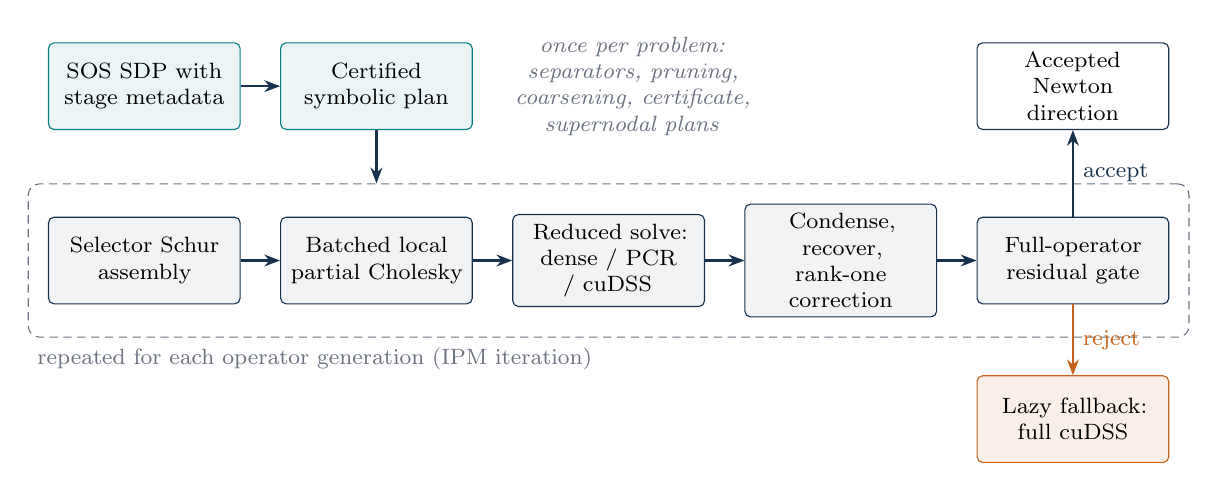
\begin{tikzpicture}[
  node distance=5mm and 5mm,
  box/.style={draw=paperblue,rounded corners=2pt,align=center,font=\footnotesize,
              minimum height=11mm,text width=22mm,fill=paperblue!6},
  setup/.style={box,draw=paperteal,fill=paperteal!8},
  fb/.style={box,draw=paperorange,fill=paperorange!10},
  arr/.style={-{Stealth[length=2mm]},thick,paperblue}]
  \node[box] (c) {Selector Schur\\assembly};
  \node[box,right=of c] (d) {Batched local\\partial Cholesky};
  \node[box,right=of d] (e) {Reduced solve:\\dense / PCR / cuDSS};
  \node[box,right=of e] (f) {Condense,\\recover, rank-one\\correction};
  \node[box,right=of f] (g) {Full-operator\\residual gate};
  \node[setup,above=11mm of c] (a) {SOS SDP with\\stage metadata};
  \node[setup,right=of a] (b) {Certified\\symbolic plan};
  \node[box,above=11mm of g,fill=white] (ipm) {Accepted\\Newton direction};
  \node[fb,below=9mm of g] (h) {Lazy fallback:\\full cuDSS};
  \node[draw=papergray,densely dashed,rounded corners,inner sep=2.5mm,
        fit=(c)(d)(e)(f)(g)] (loop) {};
  \node[font=\footnotesize,text=papergray,anchor=north west] at (loop.south west)
        {repeated for each operator generation (IPM iteration)};
  \draw[arr] (a) -- (b);
  \draw[arr] (b.south) -- (b.south |- loop.north);
  \draw[arr] (c) -- (d);
  \draw[arr] (d) -- (e);
  \draw[arr] (e) -- (f);
  \draw[arr] (f) -- (g);
  \draw[arr] (g) -- node[right,font=\footnotesize]{accept} (ipm);
  \draw[arr,paperorange] (g) -- node[right,font=\footnotesize]{reject} (h);
  \node[setup,fill=none,draw=none,text width=34mm,right=2mm of b,
        font=\footnotesize\itshape,text=papergray]
        {once per problem: separators, pruning, coarsening, certificate, supernodal plans};
\end{tikzpicture}
\caption{Structure of the SPRINT stage backend. Setup (teal) runs once per
problem. Each IPM operator generation assembles the Schur matrix, factors the
interior components in batches, solves a small reduced system, and accepts a
direction only after a residual check against the full operator; on rejection,
a lazily created full-system cuDSS factorization of the same operator is used.}
\label{fig:pipeline}
\end{figure}

\subsection{Symbolic preparation}

The customized SPOT exporter attaches stage metadata to PSD blocks, free
variables and coefficient rows, while leaving the SDP coefficients unchanged.
The metadata is used only to \emph{propose} interfaces; the assembled
conservative Schur pattern is the final authority. Initial separators come from
stage-local connectivity and vertex cuts. Carry pruning and coarsening then
propose smaller retained sets, and every proposal is accepted only after the
certificate of \cref{def:certificate} has been checked on the actual pattern.
When the last physical cut disappears, its tail joins an interior component and
the remaining groups are reindexed consecutively. CHOLMOD~\cite{chen2008cholmod}
is used for symbolic ordering only; the numerical factorization runs on arrays
owned by SPRINT. \Cref{alg:symbolic} summarizes the procedure.

\begin{algorithm}[htbp]
\caption{Symbolic preparation (once per problem)}\label{alg:symbolic}
\small
\begin{algorithmic}[1]
\Require SDP coefficient maps, conservative Schur pattern $G$, stage metadata, border $B$
\Ensure a certified structured symbolic plan, or a general-solver route
\State validate row indices, stage metadata and the complete Schur pattern
\State propose stage separators; optionally apply carry pruning and coarsening
\State form disjoint groups $R_1,\ldots,R_K$ with compact indices
\State find the components $I_j$ of $G[V\setminus R]$
\If{a retained edge or a component boundary violates \cref{def:certificate}}
  \State \Return general-solver route
\EndIf
\State build local interior/front patterns and scatter maps from the global Schur storage
\State order each interior with its retained front last; build supernodal plans
\State group components with compatible patterns; build packing and execution schedules
\State build the reduced chain/border pattern and select its solver route
\State allocate reusable buffers and publish the plan
\end{algorithmic}
\end{algorithm}

The linear-time certificate check does not bound every step of
\cref{alg:symbolic}: separator search, ordering, pattern grouping and the
current indexing structures have their own costs (\cref{app:implementation}).

\subsection{Assembly and local partial factorization}\label{sec:local-factor}

At each iterate, the solver computes the cone scalings and assembles the
numerical Schur matrix, choosing per block between sparse-coordinate selection
(\cref{prop:selector}) and a dense block path. The current implementation
assembles the global sparse matrix before packing local panels.

For component $j$, only the $A_j$ variables of the local augmented matrix
$\bigl[\begin{smallmatrix}A_j&G_j\\G_j^\top&0\end{smallmatrix}\bigr]$
are eliminated, so its retained block becomes $-G_j^\top A_j^{-1}G_j$. The
augmented matrix need not be positive definite; positive definiteness is
required only of the interior pivots and of the assembled reduced matrix. With an
optional positive diagonal equilibration $\Lambda_j$,
\begin{equation}\label{eq:local-factor}
\Lambda_jA_j\Lambda_j=L_jL_j^\top,\qquad C_j=L_j^{-1}\Lambda_jG_j,
\end{equation}
the local update is $-C_j^\top C_j$. For a right-hand side, with
$q_j=L_j^{-1}\Lambda_jf_j$, condensation and recovery are
\begin{equation}\label{eq:local-solve}
\widehat f_R=f_R-\sum_jC_j^\top q_j,\qquad x_j=\Lambda_jL_j^{-\top}(q_j-C_jx_R).
\end{equation}
These formulas describe the panel operations; no dense matrix holding the $C_j$
is formed. Equilibration is a change of coordinates and adds no regularization.

\subsection{Repeated patterns and scheduling}

Most stage interiors share the same sparsity pattern. The solver groups such
components, optionally taking a union of compatible coupling patterns with
explicit zeros, so that each group shares one symbolic plan while numerical
values and factors remain per instance. Within a plan, an update task runs once
its source panel is ready. Independent components and nonconflicting task
groups run concurrently, overlapping writes follow an explicit order, and
repeated schedules are captured as CUDA graphs to reduce launch overhead. The
retained front is an update destination throughout and is never factored as a
local pivot. Union patterns and relaxed supernodes add structural zeros, so the
cost~\eqref{eq:panel} is evaluated on the padded plans.

\subsection{Reduced system, recovery and the numerical contract}

After the local fronts are computed, the solver forms
$S=D+\sum_jF_j$ with $F_j=-G_j^\top A_j^{-1}G_j$, adding contributions to a
shared entry in a fixed order. The reduced system is solved by dense Cholesky
when it is small, by block cyclic reduction (PCR) when the certified chain and
the backend limits allow it, and by sparse cuDSS otherwise. A dense route is
consistent with the asymptotic bounds only under a size threshold independent
of~$N$, and a sparse route inherits the complexity of its own ordering. After the
retained variables are solved, the backward pass recovers the interior variables
from the same local factors, and the rank-one correction~\eqref{eq:sm} is
applied. \Cref{alg:factor,alg:solve} state the dependencies and the acceptance
contract.

\begin{algorithm}[htbp]
\caption{Numerical factorization for one operator generation}\label{alg:factor}
\small
\begin{algorithmic}[1]
\Require symbolic plan, current cone scalings, shift $\delta$
\Ensure published factors and rank-one preparation, or a reported failure
\State assemble $H_0$ and the rank-one vector $u$; form $H_\delta=H_0+\delta I$ once
\State pack local panels from $H_\delta$ and apply consistent equilibration
\State factor the interior panels (batched by template) and accumulate the retained fronts
\State check every local factor status and finite-value flag
\State assemble and factor the reduced operator on the selected route
\State if $u\ne0$, compute $v=H_\delta^{-1}u$ and $1+u^\top v$
\State validate and publish the factor generation
\Statex \emph{On failure:} invalidate all dependent state; a fallback may factor the
same operator; if the IPM changes $\delta$, restart for the new generation.
\end{algorithmic}
\end{algorithm}

\begin{algorithm}[htbp]
\caption{Checked solve with a published factor generation}\label{alg:solve}
\small
\begin{algorithmic}[1]
\Require published factors, right-hand side $f$, tolerance, refinement budget
\Ensure an accepted solution of the full operator $\Hfull x=f$, or failure
\State condense $f$ through the local forward factors
\State solve the reduced system for $x_R$; recover all interior variables
\State apply the rank-one correction of the same generation
\State compute the residual against the original full operator
\If{statuses, finite values and residual pass} \State \Return $x$ \EndIf
\State refine within the budget, or reject the route and solve the same
  operator with the lazily created fallback; report failure if no route succeeds
\end{algorithmic}
\end{algorithm}

\paragraph{Integration with the IPM.}
An accepted factorization serves several right-hand sides, but the corrector
right-hand side depends on the predictor and cannot be prepared in advance. Reuse
is therefore organized around one operator generation and a sequence of solves.
A rejected factor or a changed shift invalidates its rank-one preparation,
reduced factor and saved recovery data, and an affine direction computed for one
operator is never combined with a corrector from an incompatible factor state.

\subsection{Numerical acceptance}\label{sec:acceptance}

\Cref{thm:chain,thm:main} hold in exact arithmetic. In floating point, a valid
certificate does not prevent loss of accuracy, so the residual is computed with
the original assembled operator after recovery and the rank-one correction; a
reduced residual alone cannot detect an inaccurate condensation or recovery. For
$M=\Hfull\succ0$, $f\ne0$ and a computed $\widehat x$, let
$r_f=f-M\widehat x$ and $\eta_2=\|r_f\|_2/\|f\|_2$.

\begin{proposition}[residual interpretation]\label{prop:residual}
If $x=M^{-1}f$, then $\|\widehat x-x\|_M=\|r_f\|_{M^{-1}}$ and
$\|\widehat x-x\|_2/\|x\|_2\le\kappa_2(M)\,\eta_2$.
\end{proposition}

\begin{proof}
Since $\widehat x-x=-M^{-1}r_f$, the squared energy norm is $r_f^\top M^{-1}r_f$.
Also $\|\widehat x-x\|_2\le\|M^{-1}\|_2\|r_f\|_2$ and $\|f\|_2\le\|M\|_2\|x\|_2$.
\end{proof}

\begin{proposition}[effect of the shift]\label{prop:shift}
If $M_0=H_0+uu^\top\succ0$, $\delta\ge0$, $x_0=M_0^{-1}f$ and
$x_\delta=(M_0+\delta I)^{-1}f$, then
$\|x_\delta-x_0\|_2/\|x_0\|_2\le\delta/(\lambda_{\min}(M_0)+\delta)$.
\end{proposition}

\begin{proof}
The resolvent identity gives $x_\delta-x_0=-\delta(M_0+\delta I)^{-1}x_0$, and the
multiplying matrix has spectral norm $\delta/(\lambda_{\min}(M_0)+\delta)$.
\end{proof}

A small residual therefore does not imply a small forward error independently of
conditioning, and it does not certify feasibility or optimality for the SDP;
those remain the job of the outer termination test and of the independent
checks in \cref{sec:experiments}. Some stabilized routes factor an auxiliary
matrix $H_\delta+D_{\mathrm{priv}}$ and use it as a preconditioner for the target
system. Acceptance then uses the target operator with $D_{\mathrm{priv}}$
excluded, and the solver reports failure when the contract cannot be met.

\subsection{Choosing a hierarchy}\label{sec:select}

For a candidate retention and coarsening configuration $\theta$,
\cref{thm:main} suggests the structural estimate
\begin{equation}\label{eq:cost-model}
\widehat W(\theta)=\Phi_2(\theta)+\mathcal B_2(\theta)+K(\theta)p(\theta)^3
+K(\theta)p(\theta)^2g+K(\theta)p(\theta)g^2+g^3,
\end{equation}
in which~\eqref{eq:ragged} and~\eqref{eq:panel} can replace the conservative
terms. Coarsening usually reduces the number of groups but enlarges the
components, and pruning can shrink interfaces but increase local fill, so
separator cardinality alone is an incomplete objective. The current
implementation uses structural gates and empirically tuned thresholds. Selecting
the hierarchy automatically by minimizing~\eqref{eq:cost-model}, extended with
launch and bandwidth terms, is future work.

\section{Numerical experiments}\label{sec:experiments}

We address three questions: how MIST compares with CPU interior-point solvers at
the same or higher accuracy (\cref{sec:pushbox,sec:pendulum}); how much the
hierarchy gains over a general sparse factorization on the same GPU
(\cref{sec:cudss}); and whether the time is spent where the analysis predicts
(\cref{sec:phases}).

\subsection{Setup}\label{sec:setup}

\paragraph{Problems.}
PushT and PushBox are contact-rich planar pushing tasks from SPOT~\cite{kang2025spot};
the third problem is a three-dimensional pendulum maneuver. All are relaxed at
order $r=2$ and exported with stage labels; the largest PushT instance ($N=100$)
has $259{,}499$ equations and $63{,}885$ Gram blocks. \todo{table of instance
sizes ($m$, number and orders of Gram blocks) for all problems.}

\paragraph{Solvers and hardware.}
We compare MIST with MOSEK~11.0.10~\cite{mosek} and BRISK~1.6.5~\cite{brisk} on
the same workstation (one H100 for MIST, CPU for the baselines), and with
full-system cuDSS~0.7.1.6~\cite{cudss} inside the same IPM on one A100.
\todo{CPU model and thread counts.}

\paragraph{Accuracy and timing.}
Every returned solution is checked independently on the original SDP using eight
relative metrics: primal and dual equality residuals, duality gap,
complementarity, the distances of the primal and dual matrices to the PSD cone,
and their symmetry residuals. A solution passes the \emph{standard} check if all
metrics are below $10^{-4}$, and the \emph{strict} check if all are below
$10^{-6}$ with unaveraged complementarity. Times run from reading the problem to
writing the solution; the independent check is not timed.

\subsection{Comparison with CPU solvers}\label{sec:pushbox}

\Cref{tab:pushbox,fig:pushbox} report PushBox for horizons from 2 to 80. MIST
selects its CPU backend for $N\le5$ and the GPU backend from $N=10$ on.

\begin{table}[htbp]
\centering
\caption{PushBox: time (s, median over repeated runs) and number of runs whose
solution passes the strict $10^{-6}$ check on the original SDP.}
\label{tab:pushbox}
\small
\begin{tabular}{@{}r rrr ccc@{}}
\toprule
& \multicolumn{3}{c}{Time (s)} & \multicolumn{3}{c}{Strict check passed}\\
\cmidrule(lr){2-4}\cmidrule(l){5-7}
$N$ & MIST & BRISK & MOSEK & MIST & BRISK & MOSEK\\
\midrule
2  & 0.70 & 0.62 & 0.73 & 1/1 & 2/2 & 2/2\\
5  & 2.48 & 3.61 & 2.38 & 3/3 & 0/2 & 0/2\\
10 & 4.13 & 4.84 & 3.63 & 3/3 & 0/2 & 0/2\\
20 & \textbf{5.46} & 13.21 & 8.42 & 3/3 & 0/1 & 0/1\\
50 & \textbf{7.32} & 13.23 & 20.89 & 3/3 & 0/1 & 0/1\\
80 & \textbf{9.20} & 29.34 & 28.61 & 3/3 & 0/1 & 0/1\\
\bottomrule
\end{tabular}
\end{table}

\begin{figure}[htbp]
\centering
\begin{tikzpicture}
\begin{loglogaxis}[
  width=.68\linewidth,height=5.8cm,
  xlabel={Horizon $N$},ylabel={Time (s)},
  xmin=1.7,xmax=95,ymin=0.4,ymax=45,
  xtick={2,5,10,20,50,80},xticklabels={2,5,10,20,50,80},
  ytick={0.5,1,2,5,10,20,40},yticklabels={0.5,1,2,5,10,20,40},
  grid=both,grid style={gray!18},
  legend style={at={(0.03,0.97)},anchor=north west,draw=none,font=\small,fill=white,fill opacity=0.85,text opacity=1},
  legend cell align=left]
\addplot[paperblue,very thick,mark=*,mark size=2.4pt]
  table[x=N,y=gipm_sec,col sep=comma]{data/pushbox_strict.csv};
\addlegendentry{MIST}
\addplot[paperorange,thick,mark=square*,mark size=2.2pt,mark options={fill=white}]
  table[x=N,y=mosek_sec,col sep=comma]{data/pushbox_strict.csv};
\addlegendentry{MOSEK 11}
\addplot[paperteal,thick,densely dashed,mark=triangle*,mark size=2.8pt,mark options={fill=white,solid}]
  table[x=N,y=brisk_sec,col sep=comma]{data/pushbox_strict.csv};
\addlegendentry{BRISK 1.6.5}
\addplot[paperorange,only marks,mark=square*,mark size=2.2pt,forget plot] coordinates {(2,0.73)};
\addplot[paperteal,only marks,mark=triangle*,mark size=2.8pt,forget plot] coordinates {(2,0.62)};
\end{loglogaxis}
\end{tikzpicture}
\caption{PushBox time versus horizon. Filled markers: all runs pass the strict
check; hollow markers: none does.}
\label{fig:pushbox}
\end{figure}

For $N\le10$ the three solvers are within a factor of about 1.5, since these
instances are too small to occupy a GPU. From $N=20$ on, MIST is $1.5$--$3.1\times$
faster than MOSEK and $1.8$--$3.2\times$ faster than BRISK, and its time grows by
only $1.7\times$ from $N=20$ to $N=80$, against $3.4\times$ for MOSEK. MIST's
solutions pass the strict check in every run, whereas for $N\ge5$ no MOSEK or
BRISK solution does: MOSEK stops with its own optimality status but leaves primal
residuals and complementarity above $10^{-6}$ on the original SDP, and BRISK
reports numerical difficulties from $N=10$ on.

\subsection{A long-horizon instance: 3D pendulum}\label{sec:pendulum}

\Cref{tab:pendulum} reports the three-dimensional pendulum with $N=20$, solved by
MOSEK with eight CPU threads and by MIST on one H100.

\begin{table}[htbp]
\centering
\caption{3D pendulum, $N=20$.}
\label{tab:pendulum}
\small
\begin{tabular}{@{}lrrc@{}}
\toprule
Solver & Iterations & Solver time (s) & Converged (strict check)\\
\midrule
MOSEK (8 CPU threads) & 21 & 1{,}173.0 & yes\\
MIST (H100) & 35 & 95.1 & yes\\
\bottomrule
\end{tabular}
\end{table}

Both solvers converge. MIST takes more iterations, but each costs $2.7$\,s instead of $55.9$\,s, so it is $12.3\times$ faster overall.

\subsection{Hierarchical elimination versus general sparse factorization}\label{sec:cudss}

To isolate the hierarchy, we run the same IPM on the same A100 with two linear
backends: full-system cuDSS on the assembled $H_\delta$, and the hierarchical
backend of \cref{sec:algorithm}. Each backend ran one warm-up and three measured
runs per horizon on PushT; all runs pass the standard check, and the hierarchical
backend never fell back to cuDSS.

\begin{table}[htbp]
\centering
\caption{PushT on one A100: solver time, median [min, max] of three runs, with the
same IPM and two linear backends.}
\label{tab:cudss}
\small
\begin{tabular}{@{}rllcl@{}}
\toprule
$N$ & Full cuDSS (s) & Hierarchical (s) & Speedup & Reduced solve\\
\midrule
10  & 1.455 [1.443, 1.460] & 1.446 [1.444, 1.457] & $1.01\times$ & dense\\
30  & 3.124 [3.099, 3.125] & 2.629 [2.548, 2.633] & $1.19\times$ & dense\\
100 & 9.276 [9.134, 9.329] & 7.624 [7.612, 7.638] & $1.22\times$ & cyclic reduction\\
\bottomrule
\end{tabular}
\end{table}

The two backends tie at $N=10$, and the hierarchy is $1.19\times$ and
$1.22\times$ faster at $N=30$ and $N=100$, with similar iteration counts. These
ratios include assembly and all other IPM work, which both backends share. Since
cuDSS could in principle find an equally good ordering (\cref{prop:ordering}),
the gain comes from execution: a small reduced system, batched factorization of
identical stages, and no global sparse analysis.

\subsection{Where the time goes}\label{sec:phases}

\Cref{tab:phases} breaks down one PushT run with $N=100$ on an A100 with the
current version of MIST.

\begin{table}[htbp]
\centering
\caption{Phase times for PushT, $N=100$, one A100. Indented rows are parts of the
row above.}
\label{tab:phases}
\small
\begin{tabular}{@{}lrr@{}}
\toprule
Phase & Time (ms) & Share of Newton loop\\
\midrule
Setup (assembly structures, interfaces, symbolic plans) & 1{,}373 & --\\
Newton loop, 24 iterations & 1{,}748 & 100\%\\
\quad Local partial factorization & 618 & 35\%\\
\quad Forward condensation & 303 & 17\%\\
\quad Interior recovery & 137 & 8\%\\
\quad Reduced factorization and solves & 21.5 & 1.2\%\\
\bottomrule
\end{tabular}
\end{table}

An iteration takes about 73\,ms. The reduced system costs about $1\%$ of the
Newton loop, while local factorization, condensation and recovery dominate. This
is what \cref{thm:main} predicts once pruning and coarsening have made the
interfaces small: the cost is governed by the local front terms $\Phi_2$ and
$\Phi_1$, and that is exactly the part MIST executes as batched GPU kernels.

\section{Discussion and limitations}\label{sec:discussion}

\paragraph{What the guarantees cover.}
The linear-work results are constructive. They follow from a resource-incidence
model, an explicit temporal ordering and a certificate on the retained
hierarchy, and they bound the \emph{numerical} elimination for a fixed
regularized operator. Three costs are outside their scope. First, symbolic
setup: the current component-layout builder uses dense pair-position and
component-by-row tables of size $O(m_R^2+Jm_R)$ for $m_R=|R|$, so peak setup
memory is not yet linear (\cref{app:implementation}), and setup takes about as
long as the Newton loop at $N=100$ (\cref{tab:phases}). Second, the number of
outer iterations: we give no iteration bound for the implemented homogeneous
self-dual Mehrotra method, although the observed counts grow slowly. Third,
floating-point accuracy: exactness of condensation does not protect against
ill-conditioning, which is why every direction is checked against the full
operator and a fallback exists.

\paragraph{What the experiments show.}
The strongest results are the comparisons with MOSEK and BRISK
(\cref{sec:pushbox,sec:pendulum}), where SPRINT is faster from moderate horizons
on and, on PushBox, is the only solver that meets a strict $10^{-6}$ check on the
original SDP. They compare complete solver systems on different hardware (one
GPU versus a multicore CPU), and the baselines were measured earlier than the
current SPRINT version. The paired comparison with cuDSS (\cref{sec:cudss}) holds
the hardware and the IPM fixed. It shows a consistent but modest gain from the
hierarchy itself, which agrees with \cref{prop:ordering}: a general sparse
factorization can find comparable orderings, and the remaining advantage lies in
execution. The phase breakdown shows that the reduced system is a negligible
cost and that local partial factorization dominates, as \cref{thm:main}
predicts.

\paragraph{Future work.}
Four directions follow directly. (i) Assembling cone contributions directly into
local panels would remove the global sparse Schur matrix from the critical path.
(ii) Sparse indexing of the symbolic structures would extend the linear bounds
to total memory. (iii) Choosing the hierarchy by minimizing the cost
model~\eqref{eq:cost-model}, extended with hardware terms, would replace the
current empirical thresholds. (iv) Reusing factors across iterations, in the
spirit of inverse maintenance~\cite{jiang2022sos}, is attractive because spectral
approximation survives exact condensation without dependence on $N$
(\cref{prop:spectral}). However, a rank-one change of one scaling matrix can
induce a rank-$k$ change of the Schur matrix (\cref{prop:rank}), so cheap
updates are not automatic.

\section{Conclusion}\label{sec:conclusion}

Temporal repetition makes trajectory SOS relaxations large, but it also leaves
their coefficient resources and elimination interfaces local. We made this
precise with monomial separator bounds, an explicit linear-work ordering, and a
linear-time certificate under which interior elimination produces an exact
block-tridiagonal system with a border. The resulting cost bounds depend on
actual elimination fronts and interface widths, and they guided the design of a
GPU interior-point solver whose structured backend factors repeated local
patterns in batches and leaves only a small reduced system. In experiments, this
solver matches or exceeds the accuracy of MOSEK and BRISK and is faster from
moderate horizons on, by up to $3.2\times$ on PushBox and $12.3\times$ in solver
time on a 3D pendulum problem. We see this as evidence that interior-point
methods, combined with model-aware exact elimination on GPUs, can make
high-accuracy SOS relaxations practical for long-horizon robot trajectory
optimization. Because the analysis relies only on temporal locality, the same
approach applies to other multistage polynomial optimization problems, which we
plan to study next.


\bibliographystyle{plainnat}
\bibliography{references}

\appendix
\section{Toward factor reuse across iterations}\label{app:inverse}

\citet{jiang2022sos} develop an IPM for SOS optimization that maintains an
approximate inverse of the Hessian across iterations in an interpolant
representation. Their method exploits reuse across iterations, whereas
\cref{sec:structure,sec:hierarchy,sec:complexity} exploit temporal structure
within one iteration. SPRINT uses a block-SDP scaling representation and
recomputes numerical factors at every iteration while reusing symbolic
structure. The two results below state conditions that a future combination
would have to respect; they are derived for the operator~\eqref{eq:schur}.

\subsection{A low-rank scaling change can have larger Schur rank}

For one PSD block of order $k$, define $\mathcal L_W(X)=WXW$ and
$H_c(W)=\mathcal A_c\mathcal L_W\mathcal A_c^*$, where
$\mathcal A_c(X)=(\langle A_i^{(c)},X\rangle)_i$; this reproduces~\eqref{eq:schur}.

\begin{proposition}[rank of an induced Schur update]\label{prop:rank}
Let $W,W'\succ0$ with $\operatorname{rank}(W'-W)=\rho$, and restrict $H_c$ to its
$q_c$ incident rows. Then
\begin{equation}\label{eq:rank}
\operatorname{rank}\bigl(H_c(W')-H_c(W)\bigr)\le\min\Bigl\{q_c,\ \frac{\rho(2k-\rho+1)}2\Bigr\}.
\end{equation}
\end{proposition}

\begin{proof}
Let $C=W^{-1/2}W'W^{-1/2}\succ0$, so $\operatorname{rank}(C-I)=\rho$, and let
$\mathcal T_W(X)=W^{1/2}XW^{1/2}$, an invertible map on $\Sym^k$. Then
$\mathcal L_{W'}-\mathcal L_W=\mathcal T_W\circ(\mathcal L_C-\mathcal I)\circ\mathcal T_W$.
Diagonalize $C$ orthogonally; at least $k-\rho$ of its eigenvalues equal one. In
the induced basis of $\Sym^k$, $\mathcal L_C-\mathcal I$ multiplies coordinate
$(i,j)$ by $\lambda_i\lambda_j-1$, which vanishes when both indices lie in the
unchanged eigenspace. Its rank is therefore at most
$\frac{k(k+1)}2-\frac{(k-\rho)(k-\rho+1)}2=\frac{\rho(2k-\rho+1)}2$, and
composing with $\mathcal A_c$ and $\mathcal A_c^*$ cannot increase rank.
\end{proof}

The bound is attained in general even for $\rho=1$: with $W=I$,
$W'=I+\tau e_1e_1^\top$ ($\tau>0$) and a coefficient map spanning $\Sym^k$, the
$k$ coordinates in the first row and column change, so the Schur update has rank
$k$. Summed over many blocks, the rank of the global change can grow with $N$
whenever a fixed fraction of the blocks changes. Low rank at the level of
individual scalings therefore does not give a low-rank global update.

\subsection{Spectral approximation survives exact condensation}

\begin{proposition}[Schur-complement spectral bounds]\label{prop:spectral}
Let $H,\widetilde H\succ0$ satisfy $(1-\eta)H\preceq\widetilde H\preceq(1+\eta)H$
with $0\le\eta<1$. Then for every retained set $R$,
\begin{equation}\label{eq:spectral}
(1-\eta)\,\SR_R(H)\preceq\SR_R(\widetilde H)\preceq(1+\eta)\,\SR_R(H).
\end{equation}
\end{proposition}

\begin{proof}
Fix $x_R$. The lower inequality holds for every completion $x_I$; minimizing
over $x_I$ and using~\eqref{eq:minform} gives the lower bound. For the upper
bound, evaluate the form of $\widetilde H$ at the completion that minimizes the
form of $H$, and then minimize.
\end{proof}

A relative spectral bound on the full operator is therefore inherited by its
exact reduced operator, with no factor depending on the number of stages. Obtaining
such a bound from approximate local contributions is a separate problem:
small entrywise errors in $D$ and in the local fronts need not control their
difference $D-\sum_jG_j^\top A_j^{-1}G_j$ when it involves heavy cancellation.
A reuse policy would also have to meet the inexact-Newton requirements of the
outer method.

\section{Implementation correspondence and scope of claims}\label{app:implementation}

\Cref{tab:source} maps the mechanisms of \cref{sec:algorithm} to the SPRINT source
files. \todo{update file links to the release commit and decide whether to
include them in the submitted version.}

\begin{table}[htbp]
\centering
\caption{Mechanisms and their implementation in SPRINT.}
\label{tab:source}
\small
\begin{tabular}{@{}p{0.48\linewidth}p{0.46\linewidth}@{}}
\toprule
Mechanism & Source\\
\midrule
Stage metadata for SOS formulations & \texttt{spot-custom/gen\_*\_stage\_sos.py}\\
Stage separators, carry pruning, revalidation & \texttt{schur\_stage\_separator.hpp}\\
Interior components, retained fronts, scatter layout & \texttt{schur\_component\_layout.hpp}\\
Repeated-pattern grouping and coupling unions & \texttt{schur\_component\_groups.hpp}\\
Supernodal panels and update DAG & \texttt{schur\_supernodal\_plan.\{hpp,cpp\}}\\
Native partial factorization, condensation, recovery & \texttt{ipm\_gpu\_component\_supernodal.cu}\\
Stage backend and reduced-solver portfolio & \texttt{ipm\_gpu\_stage\_pcr.cu}\\
Shrinking-active-set cyclic reduction & \texttt{ipm\_gpu\_pcr.cu}\\
Selector assembly, rank-one term, full-operator checks & \texttt{ipm\_gpu\_schur.cu}\\
\bottomrule
\end{tabular}
\end{table}

\paragraph{Symbolic storage.}
The component-layout builder allocates a pair-position table of
$|R|^2$ entries and component-by-retained-row masks, so its storage is
$O(m_R^2+Jm_R)$ in the worst case, even though the reduced chain has only
$O(Kp^2+Kpg+g^2)$ structural entries. The supernodal plan builder also scans
pairs of candidate source and target panels. The linear storage bound of
\cref{thm:main} is therefore a statement about numerical storage, not about the
peak memory of the executable. Sparse maps indexed only by present block pairs
and component boundaries would remove these terms.

\paragraph{Scope of the main claims.}
\Cref{tab:claims} summarizes which claims are proved, which are implemented, and
which are not established.

\begin{table}[htbp]
\centering
\caption{Status of the principal claims.}
\label{tab:claims}
\small
\begin{tabular}{@{}p{0.47\linewidth}p{0.47\linewidth}@{}}
\toprule
Claim & Status\\
\midrule
The solver performs exact hierarchical elimination & Implemented: native interior partial factors, reduced solve and native recovery\\
Condensation preserves the operator & Proved in exact arithmetic under the SPD and certificate assumptions\\
Pruning and coarsening preserve a chain & Accepted only after the certificate is rechecked\\
Numerical elimination is linear in $N$ & Proved under the uniform local bounds of \cref{cor:linear}\\
Total memory is linear in $N$ & Not established; symbolic indexing can be quadratic\\
The whole IPM has logarithmic depth & Not established; \cref{cor:depth} concerns the elimination schedule\\
Numerical factors are reused across iterations & No; symbolic plans and schedules are reused\\
General sparse Cholesky is asymptotically slower & Not claimed; see \cref{prop:ordering}\\
The complete solver runs in $O(N)$ time & Not claimed; outer iterations and setup must be included\\
The relaxation certifies global optimality of the trajectory & Not implied by the linear-algebra results\\
\bottomrule
\end{tabular}
\end{table}

\section{Additional measurements}\label{app:measurements}

The measurements below come from earlier solver revisions. We report them for
completeness; they are not paired with the results of \cref{sec:experiments}.

\paragraph{Earlier H100 comparison on PushT.}
\Cref{tab:h100} shows an earlier comparison of the stage backend with full cuDSS
on one H100. Per-run records and repetition counts for this table were not
preserved, so no ranges are given. At $N=30$, the Newton phase took $1.06$\,s
for the stage route and $1.14$\,s for the direct route, so most of the
end-to-end difference at that size came from outside the Newton phase.

\begin{table}[htbp]
\centering
\caption{Earlier H100 solver times for PushT (reported values).}
\label{tab:h100}
\small
\begin{tabular}{@{}rrrr@{}}
\toprule
$N$ & Stage (s) & Full cuDSS (s) & Speedup\\
\midrule
10 & 1.96 & 2.20 & $1.12\times$\\
30 & 2.89 & 3.93 & $1.36\times$\\
100 & 8.08 & 9.28 & $1.15\times$\\
\bottomrule
\end{tabular}
\end{table}

An earlier design diagnostic at $N=30$ explains the move to native partial
factorization. Local factorization cost about $18$\,ms, but explicitly applying
$A_j^{-1}G_j$ cost $98$--$108$\,ms, against $8$\,ms for update and scatter and
$6$\,ms for the PCR factorization. Producing the reduced system therefore cost far
more than solving it. Native partial factorization replaced the explicit inverse
action by retained-front updates, and pruning with coarsening reduced the
retained dimension from $1566$ to $113$.

\paragraph{Earlier PushBox comparison with MOSEK.}
\Cref{tab:pushbox-old} reproduces an earlier PushBox comparison, reported as accepted under Rule~A, in
which SPRINT used structured assembly with full cuDSS rather than the stage
backend. \Cref{tab:pushbox} supersedes it.

\begin{table}[htbp]
\centering
\caption{Earlier PushBox comparison with MOSEK (structured assembly, full cuDSS).}
\label{tab:pushbox-old}
\small
\begin{tabular}{@{}rrrr@{}}
\toprule
$N$ & SPRINT (s) & MOSEK (s) & Speedup\\
\midrule
5 & 1.698 & 1.460 & $0.86\times$\\
10 & 2.000 & 2.407 & $1.20\times$\\
20 & 2.688 & 5.205 & $1.94\times$\\
30 & 3.436 & 7.458 & $2.17\times$\\
50 & 4.782 & 10.798 & $2.26\times$\\
\bottomrule
\end{tabular}
\end{table}

\paragraph{CPU reference runs.}
\Cref{tab:quest-cpu} lists single CPU runs of SPRINT's sparse direct backend on the
PushT instances, used to validate the exported problems and the solution path.

\begin{table}[htbp]
\centering
\caption{SPRINT CPU reference runs on PushT (Quest, single runs, Rule~A).}
\label{tab:quest-cpu}
\small
\begin{tabular}{@{}rrrrr@{}}
\toprule
$N$ & Solver (s) & Process (s) & Iterations & Largest metric\\
\midrule
10 & 4.12 & 5.44 & 23 & $7.07\times10^{-5}$\\
30 & 13.99 & 14.63 & 24 & $6.43\times10^{-5}$\\
100 & 55.37 & 58.24 & 26 & $5.10\times10^{-5}$\\
\bottomrule
\end{tabular}
\end{table}

\paragraph{MOSEK factor diagnostics.}
For a chain-anchored moment formulation, MOSEK reports factor
nonzeros of $2.36\times10^8$, $7.69\times10^8$ and $2.88\times10^9$ and factor
flop counts of $6.30\times10^{11}$, $2.12\times10^{12}$ and $1.07\times10^{13}$ at
$N=10,30,100$, giving endpoint exponents of $1.09$ and $1.23$. These runs stopped
at a five-iteration cap and use a different formulation, so they indicate
factor growth only.


\end{document}
